\begin{appendix}

\chapter{The SHA-256 Algorithm}
\label{app:hashing-algo}

The SHA-256 algorithm is a member of a set of algorithms referred to as the SHA-2 standard.
These are described in \cite{fips180-4} and consists of algorithms for producing hashes with
lengths of 224, 256, 384 and 512 bits.
The algorithms use simple operations, limited to shifts, rotates, xor, and unsigned additions,
common single-cycle operations for general purpose CPUs, in addition to a lookup-table of constants.
This allows for high-speed implementations in both software and hardware. The different SHA-2 algorithms
differ in how and with what parameters the various operations are invoked.

SHA-256 is the algorithm used in cryptocoin mining. It operates on blocks of 512~bits and keeps
a 256~bits long intermediate hash value as state. Bitcoin uses a double pass SHA-256 hash, which
first calculates the hash of a block of the data to be hashed and then hashes the hash of the first
pass.

Before the first block is processed, the initial hash value is set to a predefined
value. The entire message that is to be hashed is then padded by adding a 1~bit to
the end of the message and then appending zeroes until the length of the final block
is 448~bits. Then the length of the entire message, without padding, is added as a
64-bit big-endian integer to the end of the block.

Then, each input block is split into a 64 times 32-bit long expanded message block, where
each 32-bit word $W_j$ is defined according to the formula

\[ W_j = \left\{
	\begin{array}{l l}
		M_j & \quad j \in \left[0, 15\right]\\
		\sigma_1(W_{j - 2}) + W_{j - 7} + \sigma_0(W-{j - 15}) + W_{j - 15} & \quad j \in \left[16, 63\right]
	\end{array}
\right.\]

\noindent where $M_j$ is the $j$th word of the input message block and the functions
$\sigma_0$ and $\sigma_1$ are defined as

\[\sigma_0 = R^7(x) \oplus R^{18}(x) \oplus S^3(x)\]
\[\sigma_1 = R^{17}(x) \oplus R^{19}(x) \oplus S^{10}(x)\]

\noindent where the operator $R^n$ means right rotation by $n$ bits and $S^n$ means right shift by $n$
bits \footnote{Curiously, \cite{sha-spec} defines the operator $R$ as shift and $S$ as rotate.
We use the more intuitive definitions.}.

\subsubsection{The Compression Function}
\label{sec:sha-compr}
The compression function is the core of the SHA-256 algorithm. It uses a look-up table
of 64 constants, $K_j$, and the following functions when calculating the new intermediate
hash values:

\[Ch(x,y,z) = (x \wedge y) \oplus (\neg x \wedge z)\]
\[Maj(x, y, z) = (x \wedge y) \oplus (x \wedge z) \oplus (y \wedge z)\]
\[\Sigma_0(x) = R^2(x) \oplus R^{13}(x) \oplus R^{22}(x)\]
\[\Sigma_1(x) = R^6(x) \oplus R^{11}(x) \oplus R^{25}(x)\]

Before starting the iterations with the compression function, the intermediate
hash values from the previous message block are assigned to the variables $a$--$h$.

At the beginning of each iteration of the compression function, two temporary
values are calculated:

\[T_1 = h + \Sigma_1(e) + Ch(e, f, g) + K_j + W_j\]
\[T_2 = \Sigma_0(a) + Maj(a, b, c)\]

The new hash values are then assigned as follows:

\[\begin{array}{l}
	h \leftarrow g \\
	g \leftarrow f \\
	f \leftarrow e \\
	e \leftarrow d + T_1\\
	d \leftarrow c \\
	c \leftarrow b \\
	b \leftarrow a \\
	a \leftarrow T_1 + T_2 \\
\end{array}\]

The compression function is run 64 times, once for each word in the extended message block,
$W_j$. Afterwards, the intermediate hash for the message is updated by adding the
variables $a$--$h$ to the corresponding values of the intermediate hash values from
the previous message block.

When the final input block has been processed, the final hash is composed by
concatenating the intermediate hash values. \cite{sha-spec, fips180-4, fordypningsprosjekt}

\chapter{Measuring Performance results}

This chapter lists up all the details regarding all the performance measuring done during this thesis.
For each selected SHMAC architecture, the performance is measured by the double hashes per second.
Every architecture have been measured when running software-only hashing, when running the SHA-256 accelerator without using the DMA Module, and then with using the DMA Module. 

\section{5X4 Tile Architecture}

The first and original architecture used for measuring, as seen in figure \ref{fig:5x4-2}.
Unfortunately, while software hashing worked on all tiles, the application crashed when using the SHA-256 accelerator on more than one row.

\begin{figure}[htb]
    \centering
    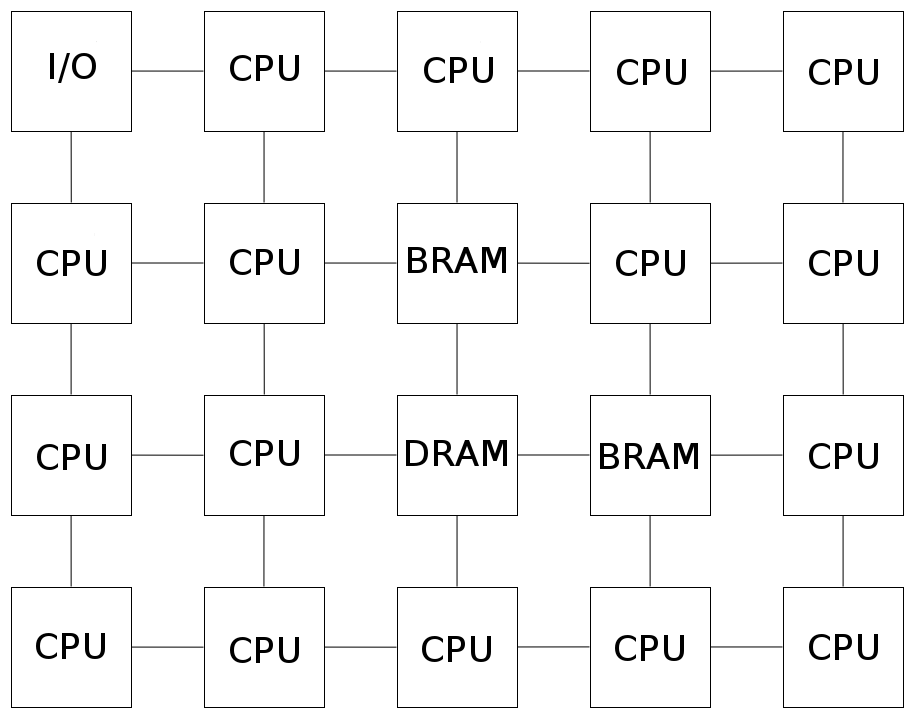
\includegraphics[width=0.5\textwidth]{Figures/Measurements/5x4}
    \caption{Test setup 1, with 5x4 architecture, using BRAM tiles as scratchpad and DRAM as main memory, placed in center.}
    \label{fig:5x4-2}
\end{figure}

\subsection{Software hashing}

The results from doing the hashing in software is listed up in table \ref{tab:Full-Perf-SW1}. 
As can be seen in the plot in figure \ref{fig:sw-scaling1} adding more processors after the third does not increase performance.

The reason for this is that all cores must make frequent accesses to DRAM, which causes the
DRAM tile to quickly become congested.

Another interesting effect to note in the results is how the XY routing affects the performance
of each tile. The more tiles that tries to access main memory through a tile, the less
performance that tile has; it seems that SHMACs router system favours requests originating
from other tiles before requests originating from the tile itself.

Exceptions are processor tile 10, which appears to have no competition with other tiles for the routing, and row 4, as adding processors from this row seems does not decrease the individual performance of other tiles. 

\begin{sidewaystable}
\begin{tabular}{| l || r r r r | r r r r | r r r | r r r r r |}
  \hline 
  \textbf{Sum} [H/s] & \textbf{0} & \textbf{1} & \textbf{2} & \textbf{3} & \textbf{4} & \textbf{5} & \textbf{6} & \textbf{7} & \textbf{8} & \textbf{9} & \textbf{10} & \textbf{11} & \textbf{12} & \textbf{13} & \textbf{14} & \textbf{15}   \\
  \hline                       
  \textbf{5972} & 5972 & - & - & - & - & - & - & - & - & - & - & - & - & - & - & - \\
  \textbf{11950} & 5971 & 5979 & - & - & - & - & - & - & - & - & - & - & - & - & - & - \\
  \textbf{17933} & 5972 & 5979 & 5982 & - & - & - & - & - & - & - & - & - & - & - & - & - \\
  \textbf{15543} & 4833 & 4701 & 2999 & 3010 & - & - & - & - & - & - & - & - & - & - & - & - \\
  \textbf{15540} & 3348 & 3339 & 1680 & 1680 & 5493 & - & - & - & - & - & - & - & - & - & - & - \\
  \textbf{15539} & 2586 & 2590 & 1297 & 1296 & 3896 & 3874 & - & - & - & - & - & - & - & - & - & - \\
  \textbf{15539} & 1796 & 1799 & 900 & 900 & 2698 & 2698 & 4748 & - & - & - & - & - & - & - & - & - \\
  \textbf{15549} & 1725 & 1728 & 865 & 864 & 2592 & 2592 & 2592 & 2591 & - & - & - & - & - & - & - & -\\
  \textbf{15536} & 1110 & 1116 & 558 & 558 & 1674 & 1675 & 1674 & 1674 & 5497 & - & - & - & - & - & - & -\\
  \textbf{15541} & 861 & 864 & 432 & 432 & 1295 & 1295 & 1295 & 1295 & 3893 & 3879 & - & - & - & - & - & -\\
  \textbf{15539} & 595 & 597 & 298 & 299 & 895 & 895 & 895 & 894 & 2684 & 2684 & 4803 & - & - & - & - & -\\
  \textbf{15537} & 434 & 435 & 217 & 218 & 652 & 652 & 653 & 653 & 1957 & 1958 & 3915 &3793 & - & - & - & -\\
  \textbf{15534} & 432 & 434 & 217 & 217 & 651 & 650 & 651 & 651 & 1953 & 1953 & 3906 & 1909 & 1910 & - & - & -\\
  \textbf{15540} & 432 & 434 & 216 & 217 & 650 & 650 & 650 & 650 & 1950 & 1949 & 3900 & 963 & 963 & 1916 & - & -\\
  \textbf{15535} & 430 & 432 & 216 & 216 & 649 & 648 & 649 & 648 & 1945 & 1946 & 3891 & 649 & 649 & 1295 & 1272 & -\\
  \textbf{16047} & 444 & 446 & 223 & 223 & 669 & 669 & 668 & 669 & 2006 & 2006 & 4012 & 669 & 669 & 1335 & 670 & 669\\
  \hline  
\end{tabular}
\caption{Software double hash results, using varying numbers of cores. Distribution on different tile-rows are highlighted by column separation}
\label{tab:Full-Perf-SW1}
\end{sidewaystable}

\begin{figure}
	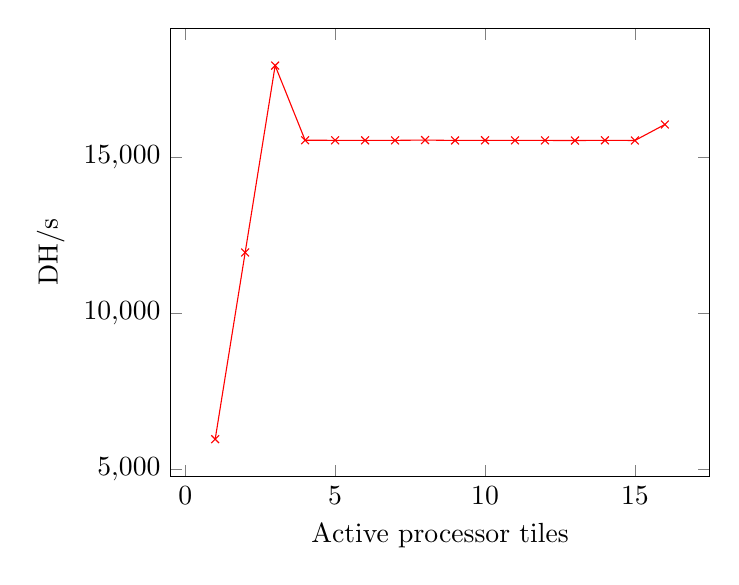
\begin{tikzpicture}
		\begin{axis}[
			xlabel=Active processor tiles,
			ylabel=DH/s,
			scaled ticks=false]
		\addplot[color=red,mark=x] coordinates {
			(1, 5972)
			(2, 11950)
			(3, 17933)
			(4, 15543)
			(5, 15540)
			(6, 15539)
			(7, 15539)
			(8, 15549)
			(9, 15536)
			(10, 15541)
			(11, 15539)
			(12, 15537)
			(13, 15534)
			(14, 15540)
			(15, 15535)
			(16, 16047)
		};
		\end{axis}
	\end{tikzpicture}
	\caption{Scaling using software hashing}
	\label{fig:sw-scaling1}
\end{figure}

\subsection{Using SHA-256 accelerator, without and with DMA, 5x4 architecture}
Tables \ref{tab:Perf-SHA1} and \ref{tab:Perf-SHADMA1} show the results when using the SHA-256 hashing accelerator, without and with DMA module, respectively.
Only up to four processors where used, as adding in processors from the second row when scaling up caused the application to crash.

\todo{Must be explained in the text}The scratchpad-bug is believed to be the cause.

Both tables shows that the sum of hashes has a near-linear increase, with very low indiviual performance drop, when scaling up.
Using DMA shows slightly increased performance for each tile.
The individual performance of each processor varies, with some higher than others, and it appaers to remain stable with the scaling. 
The application uses scratchpad tiles when the SHA-256 hashing module is in use, and positioning combined with XY-routing may be the reason behind the varying performance.

The linear increase and the comparison between the two can be seen in the plots of figure \ref{fig:shadmacomp-scaling1}, where the scaling without DMA is seen in red, and with DMA is seen in black.

\begin{table}
\begin{tabular}{| l || r r r r |}
  \hline 
  \textbf{Sum} [H/s] & \textbf{0} & \textbf{1} & \textbf{2} & \textbf{3}\\
  \hline                       
  \textbf{17541} & 17541 & - & - & - \\
  \textbf{37554} & 17527 & 20027 & - & - \\
  \textbf{54882} & 17467 & 19930 & 17485 & - \\
  \textbf{70181} & 17403 & 19882 & 17412 & 15484 \\
  \hline  
\end{tabular}
\caption{Double Hashing per second, using the SHA256-hashing module. 13x2 architecture.}
\label{tab:Perf-SHA1}
\end{table}

\begin{table}
\begin{tabular}{| l || r r r r |}
  \hline 
  \textbf{Sum} [H/s] & \textbf{0} & \textbf{1} & \textbf{2} & \textbf{3}\\
  \hline                       
  \textbf{18212} & 18212 & - & - & - \\
  \textbf{38272} & 18193 & 20079 & - & - \\
  \textbf{56142} & 18133 & 19865 & 18144 & - \\
  \textbf{71882} & 17978 & 19588 & 17988 & 16328 \\
  \hline  
\end{tabular}
\caption{Double Hashing per second, using the SHA256-hashing module and DMA module. Only up to 4 processors worked}
\label{tab:Perf-SHADMA1}
\end{table}
				
\begin{figure}
	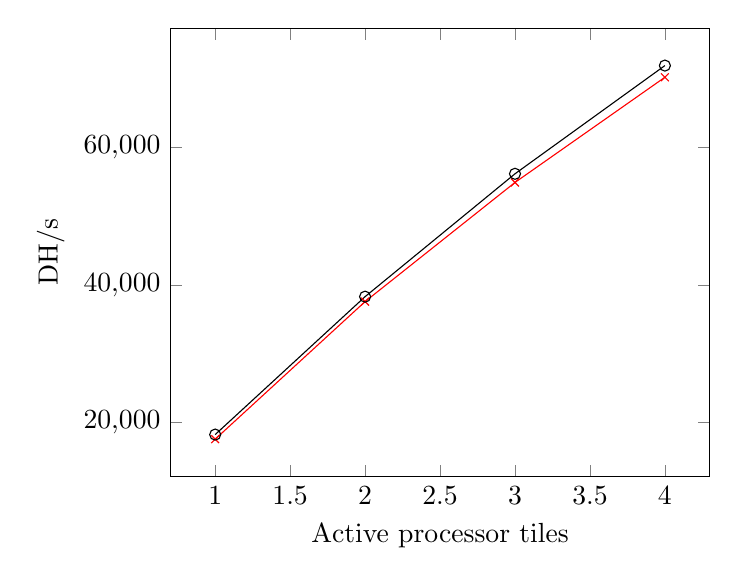
\begin{tikzpicture}
		\begin{axis}[
			xlabel=Active processor tiles,
			ylabel=DH/s,
			scaled ticks=false]
		\addplot[color=red,mark=x] coordinates {
			(1, 17541)
			(2, 37554)
			(3, 54882)
			(4, 70181)
		};
		\addplot[color=black,mark=o] coordinates {
			(1, 18212)
			(2, 38272)
			(3, 56142)
			(4, 71882)
		};
		\end{axis}
	\end{tikzpicture}
	\caption{Scaling using SHA-256 accelerator. Red: Without DMA. Black: With DMA.}
	\label{fig:shadmacomp-scaling1}
\end{figure}

\subsection{Comparison, 5x4}

The difference between software hashing and use of accelerator with DMA are compared in figure \ref{fig:comp-plot1}, where software hashing is seen in red plot, and accelerator hashing is seen in black plot.
As seen in the figure, the hashing modules greatly outperforms the software hashing, even with only up to four processors in use.

\begin{figure}
	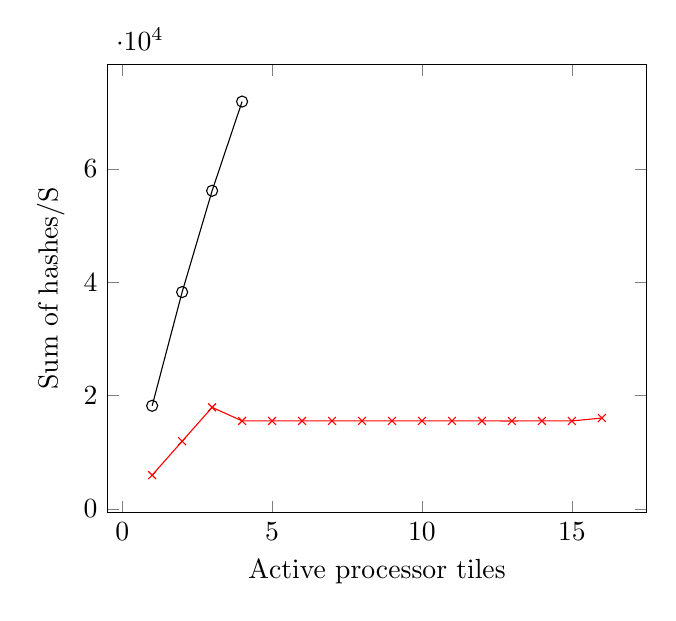
\begin{tikzpicture}
		\begin{axis}[
			xlabel=Active processor tiles,
			ylabel=Sum of hashes/S]
		\addplot[color=red,mark=x] coordinates {
			(1, 5972)
			(2, 11950)
			(3, 17933)
			(4, 15543)
			(5, 15540)
			(6, 15539)
			(7, 15539)
			(8, 15549)
			(9, 15536)
			(10, 15541)
			(11, 15539)
			(12, 15537)
			(13, 15534)
			(14, 15540)
			(15, 15535)
			(16, 16047)
		};
		\addplot[color=black,mark=o] coordinates {
			(1, 18212)
			(2, 38272)
			(3, 56142)
			(4, 71882)
		};
		\end{axis}
	\end{tikzpicture}
	\caption{Sum of double hashes per second. Red: Software only, Black: SHA-256 + DMA, 5x4 architecture}
	\label{fig:comp-plot1}
\end{figure}

\section{13X2 Tile Architecture}

Since the scratchpad-bug prevents us from measuring more than one tile, a different architecture has been synthesized and tested, as seen in figure \ref{13x2-2}.
This one circumwents the scratchpad-but by having all CPU tiles on the same upper row, while filling the second with BRAM, DRAM and empty tiles only.
This way, the use of more tiles may be measured, with the interest to find a congestion limit when using SHA-256 accelerator.
It is likely that the interconnect network may beceome congested earlier than in a different architecture, due to the XY-routing, given that the all CPU-tiles will be competing for the network on the upper row.


\begin{figure}[htb]
    \centering
    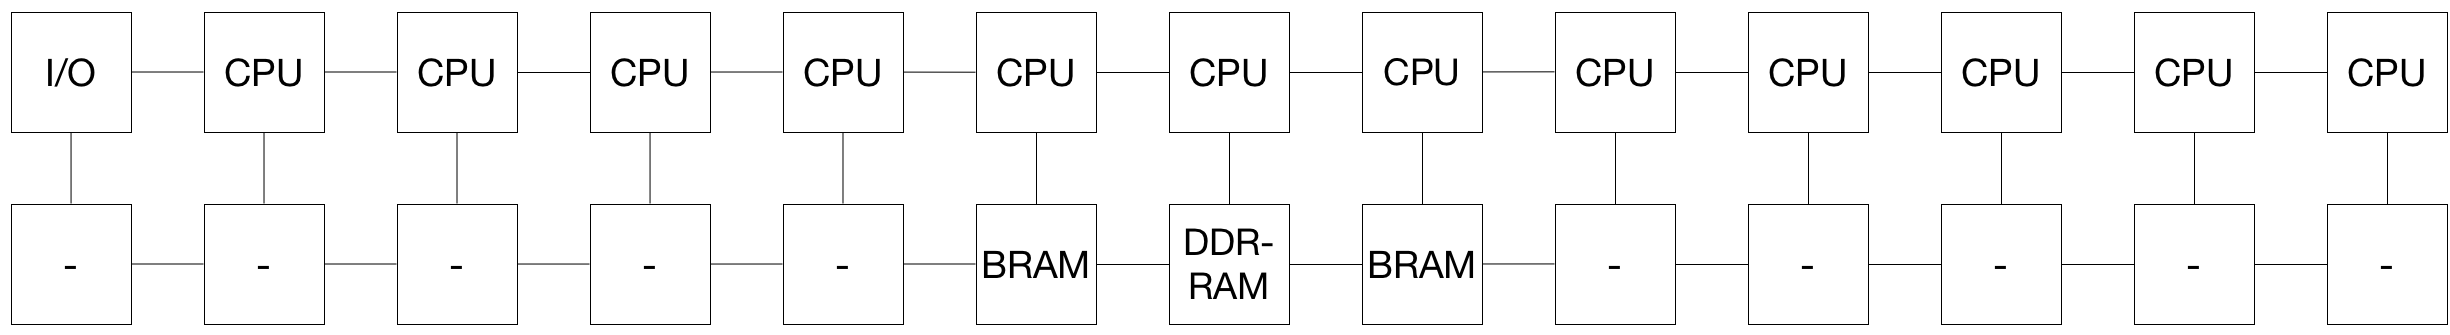
\includegraphics[width=1.0\textwidth]{Figures/Measurements/13x2}
    \caption{Test setup 2, with BRAM and DRAM tiles on second row, and all CPU's and I/O on the first row.}
    \label{fig:13x2-2}
\end{figure}

\subsection{Software Hashing, 13x2}

The results from doing the hashing in software for this architecture is listed up in table \ref{tab:Full-Perf-SW2}. 
The CPU tiles nearest the DRAM tile have highest individual performance, compared to others present.
The plot in figure \ref{fig:sw-scaling2} confirms that the pattern is the same: The application does not improve beyond three active tiles.
Once again, congested memory is the reason.



\todo{Need software hash-only data}

\begin{sidewaystable}
\begin{tabular}{| l || r r r r r r r r r r r r |}
  \hline 
  \textbf{Sum} [H/s] & \textbf{0} & \textbf{1} & \textbf{2} & \textbf{3} & \textbf{4} & \textbf{5} & \textbf{6} & \textbf{7} & \textbf{8} & \textbf{9} & \textbf{10} & \textbf{11}\\
  \hline                       
  \textbf{5963} & 5963 & - & - & - & - & - & - & - & - & - & - & - \\
  \textbf{11930} & 5962 & 5968 & - & - & - & - & - & - & - & - & - & - \\
  \textbf{17900} & 5961 & 5968 & 5971 & - & - & - & - & - & - & - & - & - \\
  \textbf{15566} & 2857 & 2840 & 4515 & 5354 & - & - & - & - & - & - & - & - \\
  \textbf{15549} & 1428 & 1431 & 2811 & 4518 & 5361 & - & - & - & - & - & - & - \\
  \textbf{15541} & 712 & 714 & 1413 & 2803 & 4523 & 5376 & - & - & - & - & - & - \\
  \textbf{15536} & 379 & 380 & 753 & 1502 & 2992 & 4723 & 4807 & - & - & - & - & - \\
  \textbf{15537} & 346 & 348 & 690 & 1376 & 2744 & 4638 & 2753 & 2642 & - & - & - & -\\
  \textbf{15536} & 345 & 347 & 688 & 1371 & 2736 & 4635 & 2744 & 1373 & 1297 & - & - & -\\
  \textbf{15534} & 344 & 346 & 686 & 1368 & 2729 & 4632 & 2736 & 1366 & 685 & 642 & - & -\\
  \textbf{15535} & 344 & 345 & 685 & 1365 & 2723 & 4627 & 2731 & 1363 & 681 & 344 & 327 & -\\
  \textbf{15536} & 344 & 345 & 684 & 1362 & 2718 & 4630 & 2726 & 1360 & 680 & 342 & 173 & 172\\
  \hline  
\end{tabular}
\caption{Software double hash results, this time on the 13x2 architecture}
\label{tab:Full-Perf-SW2}
\end{sidewaystable}


\begin{figure}
	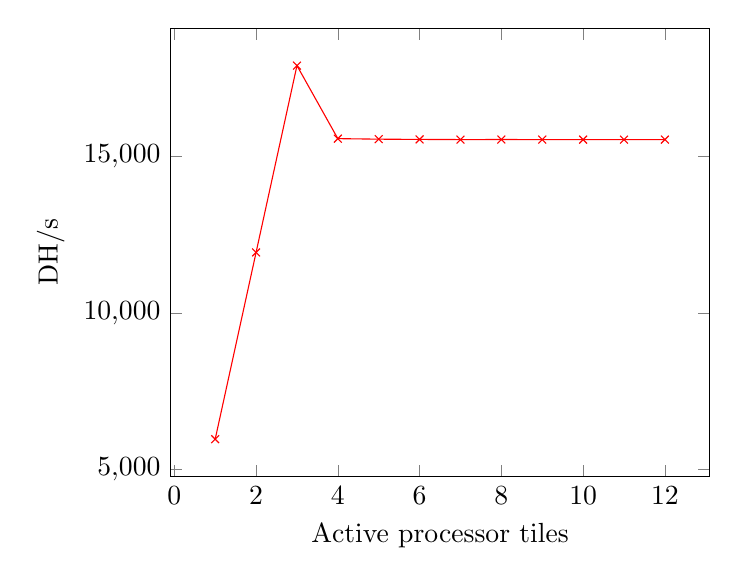
\begin{tikzpicture}
		\begin{axis}[
			xlabel=Active processor tiles,
			ylabel=DH/s,
			scaled ticks=false]
		\addplot[color=red,mark=x] coordinates {
			(1, 5963)
			(2, 11930)
			(3, 17900)
			(4, 15566)
			(5, 15549)
			(6, 15541)
			(7, 15536)
			(8, 15537)
			(9, 15536)
			(10, 15534)
			(11, 15535)
			(12, 15536)
		};
		\end{axis}
	\end{tikzpicture}
	\caption{Scaling using software hashing, 13x2 architecture}
	\label{fig:sw-scaling2}
\end{figure}

\subsection{Using SHA-256 accelerator, without and with DMA, 13x2 architecture}

Tables \ref{tab:Perf-SHA2} and \ref{tab:Perf-SHADMA2} show the results when using the SHA-256 hashing accelerator in the 13x2 architecture, without and with DMA module, respectively.
This time, using an architecture that circumvents the cache-bug problem, all available CPU's were functioning when using the SHA-256 accelerator.

The trend is the same, with a near-linear increase.
It may be observed from the table results that the closer a specific tile is in proximity to the BRAM-tiles, the higher the individual performance, with highest performance observed at CPU tiles 3-5.
This counts for both without and with DMA. 
The plots in figure \ref{fig:shadmacomp-scaling2} seems to confirm this trend: The increase become greater as the processors closer to the middle become active, and lessens beyond that point.
Unfortunately, there were not enough CPU-tiles for this architecture to find a possible saturation point.

An interesting observation is that as more tiles are added, the gain from using the DMA is reduced per tile.
The increase on CPU tile 0 is reduced from about 1500 double hashes to about mere 130.
As all CPU tiles become active, CPU tiles 1-4 have less performace compared to running without DMA, with CPU tile 4 having the biggest drop of nearly 2300 double hashes. 
CPU tiles 5-11 shows a steady increase again, up to about 1000 double hashes per second.

Judging from the positions in figure \ref{fig:13x2-2}It seems that the closer a CPU tile is to the leftmost BRAM-tile, from left (CPU tile 4 is right above), the more negative the use of DMA is.


\begin{sidewaystable}
\begin{tabular}{| l || r r r r r r r r r r r r |}
  \hline 
  \textbf{Sum} [H/s] & \textbf{0} & \textbf{1} & \textbf{2} & \textbf{3} & \textbf{4} & \textbf{5} & \textbf{6} & \textbf{7} & \textbf{8} & \textbf{9} & \textbf{10} & \textbf{11}\\
  \hline                       
  \textbf{12756} & 12756 & - & - & - & - & - & - & - & - & - & - & - \\
  \textbf{26751} & 12735 & 14016 & - & - & - & - & - & - & - & - & - & - \\
  \textbf{42268} & 12713 & 13993 & 15562 & - & - & - & - & - & - & - & - & - \\
  \textbf{59689} & 12688 & 13953 & 15526 & 17522 & - & - & - & - & - & - & - & - \\
  \textbf{79461} & 12637 & 13889 & 15456 & 17442 & 20037 & - & - & - & - & - & - & - \\
  \textbf{96589} & 12577 & 13820 & 15376 & 17352 & 19941 & 17523 & - & - & - & - & - & - \\
  \textbf{111491} & 12512 & 13748 & 15292 & 17245 & 19840 & 17391 & 15463 & - & - & - & - & - \\
  \textbf{124567} & 12440 & 13671 & 15200 & 17138 & 19740 & 17267 & 15336 & 13775 & - & - & - & -\\
  \textbf{136162} & 12375 & 13595 & 15107 & 17030 & 19642 & 17134 & 15207 & 13654 & 12418 & - & - & -\\
  \textbf{146476} & 12309 & 13520 & 15017 & 16923 & 19543 & 16987 & 15065 & 13528 & 12300 & 11284 & - & -\\
  \textbf{155681} & 12246 & 13445 & 14929 & 16818 & 19447 & 16822 & 14928 & 13385 & 12172 & 11163 & 10326 & -\\
  \textbf{164011} & 12199 & 13380 & 14848 & 16723 & 19356 & 16718 & 14774 & 13232 & 12031 & 11034 & 10204 & 9512\\
  \hline  
\end{tabular}
\caption{Double Hashing per second, using the SHA256-hashing accelerator. 13x2 architecture.}
\label{tab:Perf-SHA2}
\end{sidewaystable}

\begin{sidewaystable}
\begin{tabular}{| l || r r r r r r r r r r r r |}
  \hline 
  \textbf{Sum} [H/s] & \textbf{0} & \textbf{1} & \textbf{2} & \textbf{3} & \textbf{4} & \textbf{5} & \textbf{6} & \textbf{7} & \textbf{8} & \textbf{9} & \textbf{10} & \textbf{11}\\
  \hline                       
  \textbf{14231} & 14231 & - & - & - & - & - & - & - & - & - & - & - \\
  \textbf{29577} & 14221 & 15356 & - & - & - & - & - & - & - & - & - & - \\
  \textbf{46143} & 14175 & 15308 & 16660 & - & - & - & - & - & - & - & - & - \\
  \textbf{64070} & 14108 & 15233 & 16574 & 18155 & - & - & - & - & - & - & - & - \\
  \textbf{83379} & 13996 & 15096 & 16403 & 17968 & 19916 & - & - & - & - & - & - & - \\
  \textbf{101428} & 13837 & 14928 & 16226 & 17766 & 19617 & 19054 & - & - & - & - & - & - \\
  \textbf{117158} & 13664 & 14734 & 16007 & 17500 & 19322 & 18794 & 17137 & - & - & - & - & - \\
  \textbf{130772} & 13457 & 14511 & 15742 & 17206 & 18954 & 18551 & 16893 & 15458 & - & - & - & -\\
  \textbf{142451} & 13214 & 14232 & 15435 & 16874 & 18550 & 18257 & 16643 & 15232 & 14014 & - & - & -\\
  \textbf{152096} & 12914 & 13915 & 15118 & 16502 & 18064 & 17890 & 16277 & 14916 & 13742 & 12758 & - & -\\
  \textbf{160117} & 12622 & 13595 & 14764 & 16165 & 17556 & 17472 & 15916 & 14566 & 13438 & 12497 & 11526 & -\\
  \textbf{167103} & 12331 & 13298 & 14444 & 15907 & 17060 & 17020 & 15668 & 14257 & 13134 & 12181 & 11245 & 10558\\
  \hline  
\end{tabular}
\caption{Double Hashing per second, using the SHA256-hashing accelerator with the DMA module. 13x2 architecture.}
\label{tab:Perf-SHADMA2}
\end{sidewaystable}
		
		
			
\begin{figure}
	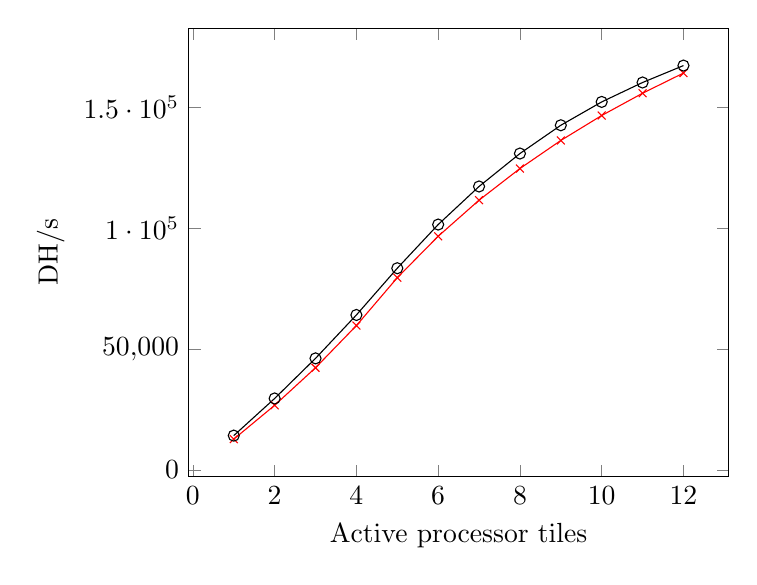
\begin{tikzpicture}
		\begin{axis}[
			xlabel=Active processor tiles,
			ylabel=DH/s,
			scaled ticks=false]
		\addplot[color=red,mark=x] coordinates {
			(1, 12756)
			(2, 26751)
			(3, 42268)
			(4, 59689)
			(5, 79461)
			(6, 96589)
			(7, 111491)
			(8, 124567)
			(9, 136162)
			(10, 146476)
			(11, 155681)
			(12, 164011)
		};
		\addplot[color=black,mark=o] coordinates {
			(1, 14231)
			(2, 29577)
			(3, 46143)
			(4, 64070)
			(5, 83379)
			(6, 101428)
			(7, 117158)
			(8, 130772)
			(9, 142451)
			(10, 152096)
			(11, 160117)
			(12, 167103)
		};
		\end{axis}
	\end{tikzpicture}
	\caption{Sum of double hashes per second. Red: Software only, Black: SHA-256 + DMA. 13x2 architecture.}
	\label{fig:shadmacomp-scaling2}
\end{figure}


\subsection{Comparison, 13x2}

Cannot compare without software hashes in figure \ref{fig:comp-plot2}.

\begin{figure}
	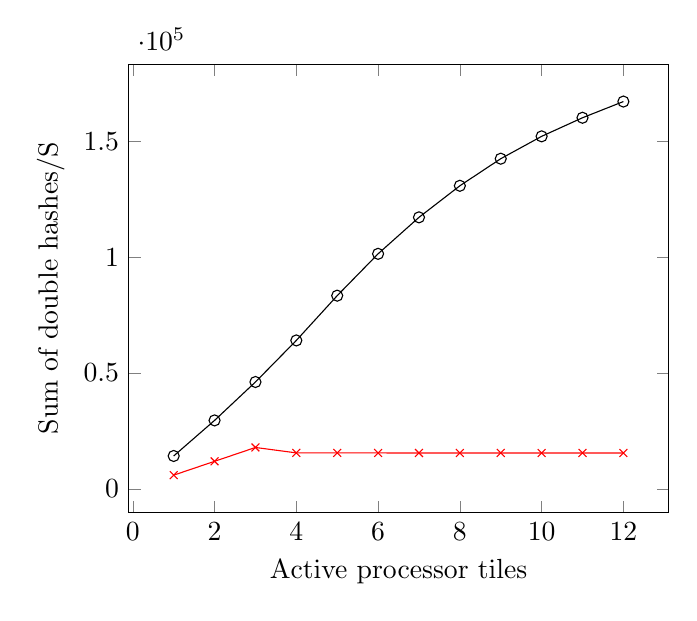
\begin{tikzpicture}
		\begin{axis}[
			xlabel=Active processor tiles,
			ylabel=Sum of double hashes/S]
		\addplot[color=red,mark=x] coordinates {
			(1, 5963)
			(2, 11930)
			(3, 17900)
			(4, 15566)
			(5, 15549)
			(6, 15541)
			(7, 15536)
			(8, 15537)
			(9, 15536)
			(10, 15534)
			(11, 15535)
			(12, 15536)
		};
		\addplot[color=black,mark=o] coordinates {
			(1, 14231)
			(2, 29577)
			(3, 46143)
			(4, 64070)
			(5, 83379)
			(6, 101428)
			(7, 117158)
			(8, 130772)
			(9, 142451)
			(10, 152096)
			(11, 160117)
			(12, 167103)
		};
		\end{axis}
	\end{tikzpicture}
	\caption{Sum of hashes per second. Red: Software only, Black: SHA-256 + DMA, 13x2 architecture}
	\label{fig:comp-plot2}
\end{figure}



\chapter{Power measurements}

For a chosen architecture, and for a set of active CPU's, the power was measured.
Compared to performance measuring, only a set of configurations were tested this time, in order to simplify the testing, and due to the pattern of the testing.

Interestingly, it turned out that the less tiles were active, the more power was consumed.
Originally, the 13x2 architecture was measured first, since it was already set up and ready on the SHMAC at the time, but to keep the consistency of this document, 5x4 will be explained first.
But due to the trend discovered in the power usage, only 1 and 16 tiles were activated for the 5x4 architecture.

It should be noted that idle power varied from time to time.
Three different numbers were measured:
31.3 W, 31.7 W and 32.3 W.

We select 31.3 W as Idle, assuming worst case usage of power.

Both power usage and uncertainty is listed up in Watt.

\section{5x4 Architecture}
 
Only software hashing was measured for power usage, since the scratchpad bug would have prevented the use of more than 4 tiles when running the SHA-256 accelerators.

Table \ref{tab:SW-power1} shows the measured power used, while \ref{fig:SW-power1} shows the plotting.

\begin{table}
\begin{tabular}{| l | r | r |}
  \hline 
  \textbf{Cores} & \textbf{Power} & \textbf{Uncertainty} \\
  \hline                       
  \textbf{IDLE} &  31.3 & 0.3 \\
  \textbf{1} &  35.0 & 0.4\\
  \textbf{16} &  33.0 & 0.4 \\
  \hline 
\end{tabular}
\caption{Measured power usage in Watts, software only, 5x4 architecture.}
\label{tab:SW-power1}
\end{table}

\begin{figure}
	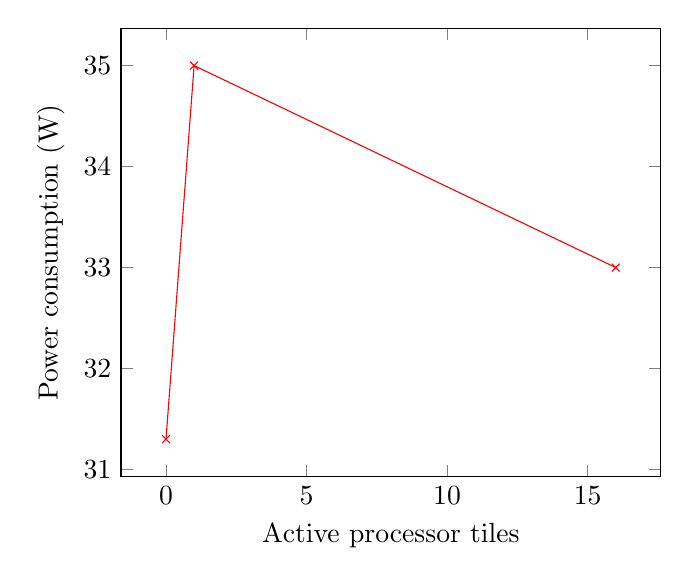
\begin{tikzpicture}
		\begin{axis}[
			xlabel=Active processor tiles,
			ylabel=Power consumption (W),
			scaled ticks=false]
		\addplot[color=red,mark=x] coordinates {
			(0, 31.3)
			(1, 35.0)
			(16, 33.0)
			
		};
		\end{axis}
	\end{tikzpicture}
	\caption{Power scaling using software hashing, 5x4 architecture}
	\label{fig:SW-power1}
\end{figure}

\section {13x2 Architecture}
For this architecture, all tiles from 0-11 were activated one by one, and measured, when running both the SHA-256 accelerator and the DMA Module.
Only a selected number for software hashing and accelerator without DMA were measured, since the power usage trend were identified and assumed for the rest of the \todo{I still think we should give this full coverage, by measuring everything} measurements.

To keep the consistency in this document, software hashing results will be detailed first, then accelerator, then accelerator with DMA.

\subsection{Software hashing power consumption, 13x2 Architecture.}

Table \ref{tab:SW-power2} and figure \ref{fig:SW-power2} shows the measured power.
Only 1, 5 and 12 tiles were measured.

\begin{table}
\begin{tabular}{| l | r | r |}
  \hline 
  \textbf{Cores} & \textbf{Power} & \textbf{Uncertainty} \\
  \hline                       
  \textbf{IDLE} &  31.3 & 0.3 \\
  \textbf{1} &  34.0 & 0.3\\
  \textbf{5} &  32.5 & 0.5\\
  \textbf{12} &  32.5 & 0.5 \\
  \hline 
\end{tabular}
\caption{Measured power usage in Watts, software only, 13x2 architecture.}
\label{tab:SW-power2}
\end{table}

\begin{figure}
	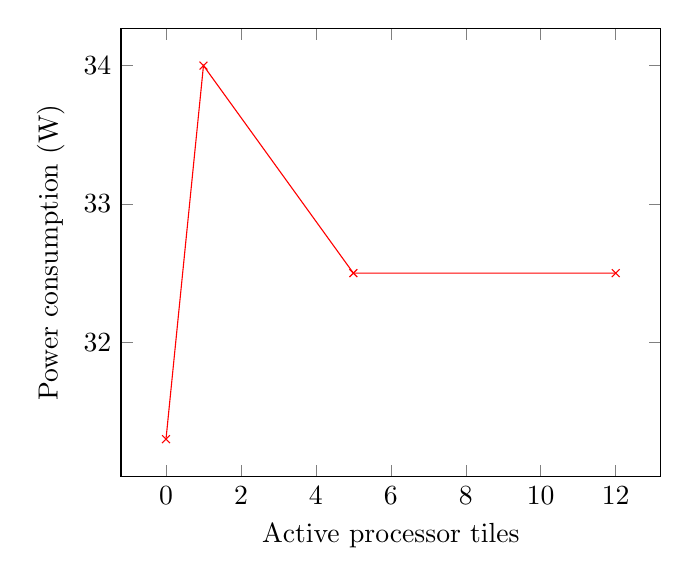
\begin{tikzpicture}
		\begin{axis}[
			xlabel=Active processor tiles,
			ylabel=Power consumption (W),
			scaled ticks=false]
		\addplot[color=red,mark=x] coordinates {
			(0, 31.3)
			(1, 34.0)
			(5, 32.5)
			(12, 32.5)
		};
		\end{axis}
	\end{tikzpicture}
	\caption{Power scaling using software hashing, 13x2 architecture}
	\label{fig:SW-power2}
\end{figure}

\subsection{SHA-256 accelerator power consumption, 13x2 Architecture.}

Table \ref{tab:SHA-power2} and figure \ref{fig:SHA-power2} shows the measured power.
Only 5 and 12 tiles were measured.

\begin{table}
\begin{tabular}{| l | r | r |}
  \hline 
  \textbf{Cores} & \textbf{Power} & \textbf{Uncertainty} \\
  \hline                       
  \textbf{IDLE} &  31.3 & 0.3 \\
  \textbf{5} &  33.7 & 0.3\\
  \textbf{12} &  32.3 & 0.5 \\
  \hline 
\end{tabular}
\caption{Measured power usage in Watts, SHA-256 accelerator, 13x2 architecture.}
\label{tab:SHA-power2}
\end{table}


\begin{figure}
	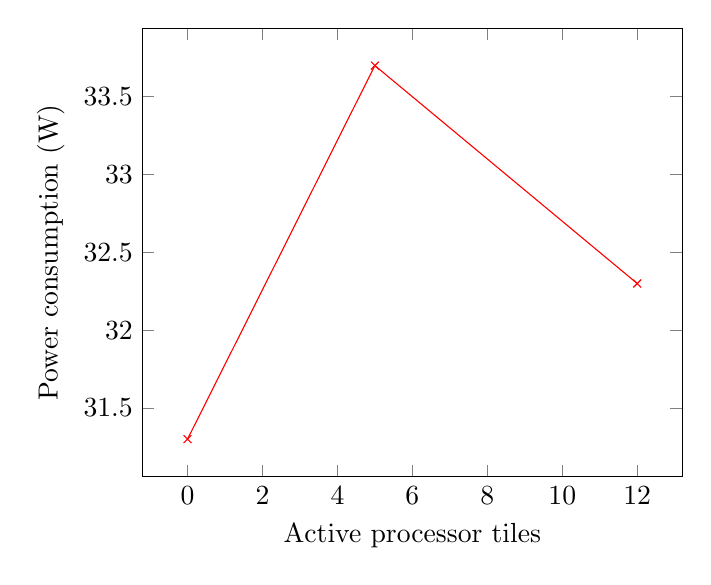
\begin{tikzpicture}
		\begin{axis}[
			xlabel=Active processor tiles,
			ylabel=Power consumption (W),
			scaled ticks=false]
		\addplot[color=red,mark=x] coordinates {
			(0, 31.3)
			(5, 33.7)
			(12, 32.3)
		};
		\end{axis}
	\end{tikzpicture}
	\caption{Power scaling using SHA-256 accelerator, 13x2 architecture}
	\label{fig:SHA-power2}
\end{figure}

\subsection{SHA-256 accelerator with DMA power consumption, 13x2 Architecture.}

This is the first series of power measurements, and all anvailable number of active tiles, from 1-12, were measured.
This laid the basis for the other measurements, as it showed the trend of the measured power usage slightly reducing as more cores are activated.
 
Unsurprisingly, using the DMA requires more power, and since the current software relies on polling the DMA, the processor is kept active.
Sleep mode does not \todo{Must get documented} exist either for Turbo Amber, so in this case it is unavoidable.

Table \ref{tab:SHADMA-power2} and figure \ref{fig:SHADMA-power2} shows the measured power.

\begin{table}
\begin{tabular}{| l | r | r |}
  \hline 
  \textbf{Cores} & \textbf{Power} & \textbf{Uncertainty} \\
  \hline                       
  \textbf{IDLE} &  31.3 & 0.3 \\
  \textbf{1} &  33.7 & 0.4\\
  \textbf{2} &  33.7 & 0.4\\
  \textbf{3} &  33.9 & 0.4\\
  \textbf{4} &  34.0 & 0.3\\
  \textbf{5} &  34.0 & 0.4\\
  \textbf{6} &  33.7 & 0.4\\
  \textbf{7} &  33.7 & 0.4\\
  \textbf{8} &  33.6 & 0.4\\
  \textbf{9} &  33.8 & 0.4\\
  \textbf{10} &  33.6 & 0.3\\
  \textbf{11} &  34.0 & 0.3\\
  \textbf{12} &  33.5 & 0.5 \\
  \hline 
\end{tabular}
\caption{Measured power usage in Watts, SHA-256 accelerator with DMA, 13x2 architecture.}
\label{tab:SHADMA-power2}
\end{table}

\begin{figure}
	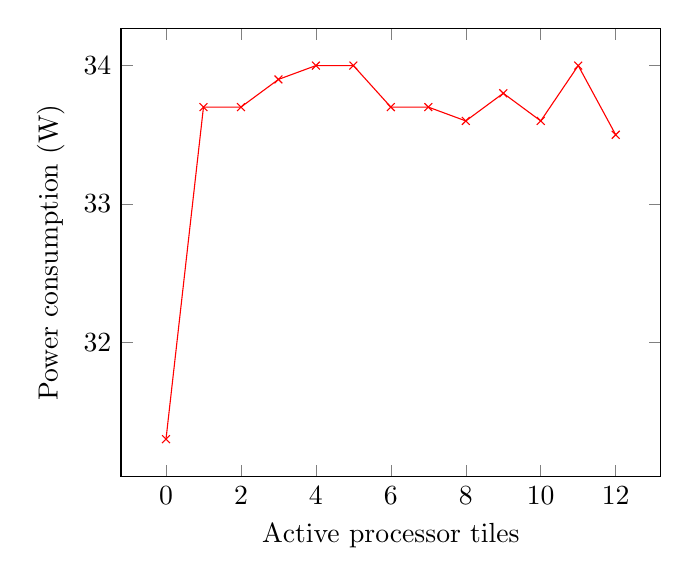
\begin{tikzpicture}
		\begin{axis}[
			xlabel=Active processor tiles,
			ylabel=Power consumption (W),
			scaled ticks=false]
		\addplot[color=red,mark=x] coordinates {
			(0, 31.3)
			(1, 33.7)
			(2, 33.7)
			(3, 33.9)
			(4, 34.0)
			(5, 34.0)
			(6, 33.7)
			(7, 33.7)
			(8, 33.6)
			(9, 33.8)
			(10, 33.6)
			(11, 34.0)
			(12, 33.5)
		};
		\end{axis}
	\end{tikzpicture}
	\caption{Power scaling using SHA-256 accelerator  with DMA, 13x2 architecture}
	\label{fig:SHADMA-power2}
\end{figure}

\chapter{Calculated Watt per Hash}


%\chapter{Detailed DMA Description}
%\label{app:DMA-arch}


\end{appendix}

